\documentclass[a4paper,12pt]{article}
\usepackage[utf8]{inputenc}
\usepackage[slovene]{babel}
\usepackage{amsmath}
\usepackage{tikz}
\usepackage{graphicx}
\usepackage{geometry}
\usepackage{titlepic}
\usepackage{spreadtab}
\usepackage{siunitx}
\usepackage{booktabs}
\usepackage{float}
\usepackage{hyperref}
\usepackage{listings}
\usepackage{xcolor}
\usepackage{caption}
\usepackage{subcaption}
\usepackage{fancyhdr}
\usepackage{tcolorbox}
\usepackage{cleveref}
\graphicspath{ {assets/} }
\usepackage{array}


% Modern color scheme
\definecolor{linkcolor}{HTML}{000000}
\definecolor{codebackground}{HTML}{F5F5F5}
\definecolor{codecomment}{HTML}{008000}
\definecolor{codekeyword}{HTML}{0000FF}
\definecolor{codestring}{HTML}{A31515}

% Page settings
\geometry{margin=2.5cm}
\hypersetup{
    colorlinks=true,
    linkcolor=linkcolor,
    filecolor=linkcolor,      
    urlcolor=linkcolor,
    citecolor=linkcolor,
}

% Code listing configuration
\lstset{
    backgroundcolor=\color{codebackground},
    commentstyle=\color{codecomment},
    keywordstyle=\color{codekeyword},
    stringstyle=\color{codestring},
    basicstyle=\ttfamily\small,
    breakatwhitespace=false,
    breaklines=true,
    captionpos=b,
    frame=single,
    numbers=left,
    numbersep=5pt,
    showspaces=false,
    showstringspaces=false,
    showtabs=false,
    tabsize=2,
    language=Python
}

% Header and footer
\pagestyle{fancy}
\fancyhf{}
\renewcommand{\headrulewidth}{0.4pt}
\renewcommand{\footrulewidth}{0.4pt}
\fancyhead[L]{\textit{Razvoj programa za kategorizacijo spojin}}
\fancyhead[R]{\textit{Martin Hanzlowsky}}
\fancyfoot[C]{\thepage}


\renewcommand\lstlistingname{Izsek kode}


\title{\LARGE{\textbf{Razvoj programa za kategorizacijo spojin}}}
\author{Martin Hanzlowsky, G 4. a}
\date{}

\begin{document}
% Title page
\begin{titlepage}

\includegraphics[scale=1]{assets/logotip_vegova_leze_brezokvirja.png}\\
\begin{center}
\vfill \Huge{ Krmiljenje, regulacije, nadzor procesov} \\\large{Razvoj programa za kategorizacijo spojin}
\normalsize
\vfill Mentor: Mentor: Aleš Volčini, prof. \hfill Avtor: Martin Hanzlowsky, G 4. A\\
\null Ljubljana, april 2025
\end{center}
\thispagestyle{empty}
\end{titlepage}

\pagenumbering{arabic}
\setcounter{page}{1}

% Abstract
\begin{tcolorbox}[title=Povzetek, colback=white, colframe=black, colbacktitle=white, coltitle=black]
V seminarski nalogi predstavljam razvoj programa za generiranje nadzornih datotek za robota Janus G3 proizvajalca Perkin Elmer. Glavni cilj je bil razviti orodje za evalvacijo izhodnega grafa masnega spektrometra ter generiranje premikov za robotsko pipetiranje. Program omogoča označevanje ključnih vrhov v spektrogramu in ustvarja datoteko v kateri so zapisana navodila za premikanje v formatu CSV.

\vspace{0.3cm}
\noindent\textbf{Ključne besede:} masni spektrometer, robotsko pipetiranje, python, nadzor naprav
\end{tcolorbox}
\thispagestyle{empty}
\newpage
% Table of contents
\tableofcontents
\thispagestyle{empty}
\listoffigures
\cleardoublepage


% Main content
\section{Uvod}
Ideja za program se je rodila pri iskanju rešitve za praktičen problem. V podjetju se je pokazala potreba po avtomatizaciji zbiranja nizkokoličinskih spojin, ki se ločijo pri masni spektrometriji. Za nadaljnjo identifikacijo spojin so potrebne večje količine, zato bi bilo potrebno proces avtomatizirati. Vendar kljub visokim donosom proizvajalcev laboratorijske opreme ostaja veliko odprtih problemov. Integracija med laboratorijskimi napravami različnih proizvajalcev je zapletena, rešitve proizvajalcev (t.i. first-party solutions) pa so še dražje, zato je pogosto v znanstvenih okoljih potrebno poiskati ali celo izdelati edinstvene rešitve.

Sprva sem načrtoval reševanje problema z nizkocenovnim mikrokrmilnikom ESP32, s katerim bi meril analogni izhod UV-spektrometra ter s tem ločil različne spojine, ki so se ločile v koloni. Zaradi različnih razlogov se je prioritizirala izdelava programa, s katerim bi na grafu prvega - pilotnega zagona masnega spektrometra označil ekstreme oziroma interesne dele. Nato bi se izdelala vodilna datoteka v .csv obliki, ki se lahko uporabi v WinPREP programski opremi za vnos oziroma kontrolo metod ki jih določi uporabnik, oziroma omogoča programiranje premikov JanusG3 pipetirnega robota. Za izdelavo programa sem najprej dobil jasne zahteve ter želje in se lotil načrtovanja.
\begin {figure}[H]
\centering
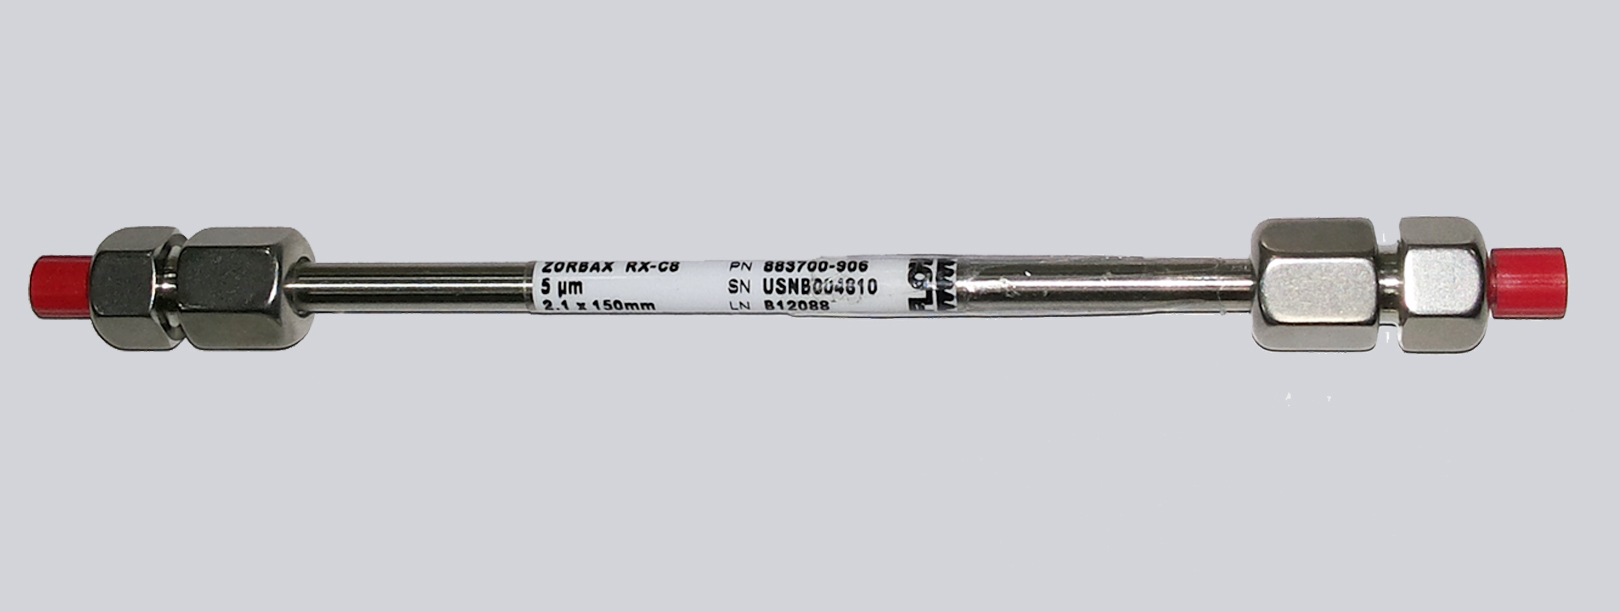
\includegraphics[width=0.8\textwidth]{assets/kolona-1.jpg}
   \caption{Kolona}
    \label{fig:kolona-1}
\end{figure}

%\begin{figure}[H]
%    \centering
%    \includegraphics[width=0.8\textwidth]{example-image}
%    \caption{Diagram poteka dela z razvitim programom. Prikazuje pot od zajema podatkov iz masnega spektrometra do kontrole JanusG3 robota.}
%    \label{fig:workflow}
%\end{figure}

\newpage
\section{Izbira programskega jezika in okolja}

Zaradi znanstvene narave projekta se je izbira Pythona kot glavnega razvojnega jezika zdela samoumevna, saj se pri procesiranju podatkov pitonski ekosistem resnično izkaže. Python tudi pripomore k hitremu razvijanju; zlahka sem preuredil in dodelal program, ko se je izkazala potreba po popravkih, kar ni zahtevalo veliko časovnih vložkov, kot bi jih zahtevala uporaba nižjenivojskih jezikov.

Iz enakih razlogov sem za razvoj grafičnega uporabniškega vmesnika (GUI) izbral kombinacijo matplotlib\cite{matplotlib} vizualizacijske knjižnice ter Tk grafičnega kompleta za razvoj uporabniških vmesnikov. Python na privzeti namestitvi podpira TK/Tcl preko vmesnika tkinter\cite{tkinter}, kar pripomore k enotni, kratki, vendar funkcionalni kodi.

\section{Struktura in funkcionalnost programa}

Osrednja funkcionalnost aplikacije je prikaz zajetih grafov masnega spektrometra ter način označevanja in kategorizacija spojin oziroma izbor ciljnih destinacij Janus G3 robota. Grafi so izrisani s pomočjo funkcij \texttt{matplotlib.pyplot.imshow} ter \texttt{PIL.Image.open}, ki skupaj omogočata odpiranje, procesiranje in prikaz vseh splošnih slikovnih datotečnih formatov.

\begin{figure}[H]
    \centering
    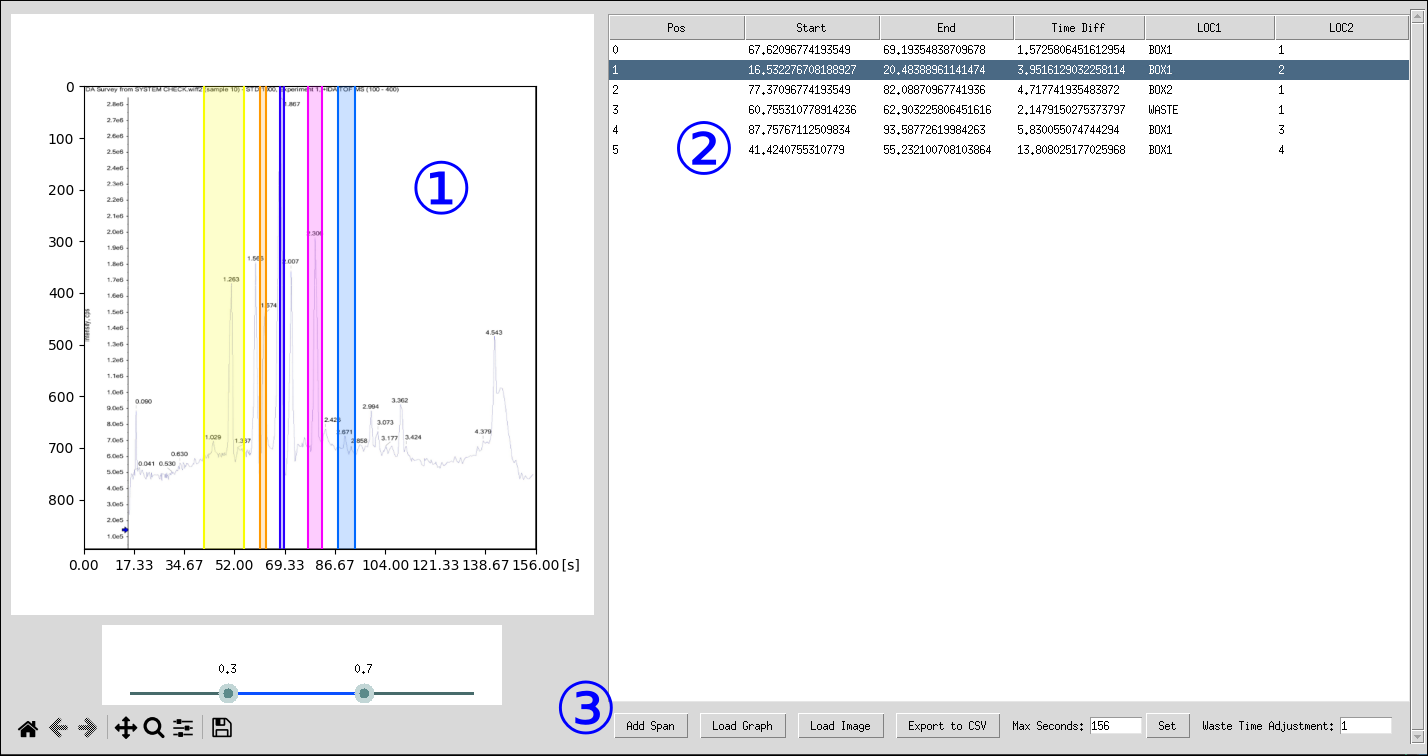
\includegraphics[width=\textwidth]{assets/full-1.png}
    \caption[Uporabniški vmesnik programa]{Uporabniški vmesnik programa  z označenimi glavnimi funkcionalnimi elementi: 1) Panel za označevanje regij, 2) Tabela označenih regij, 3) Kontrolni gumbi.}
    \label{fig:ui_overview}
\end{figure}

\subsection{Označevanje regij}

Za označevanje lokalnih maksimumov med ekstremi oziroma interesnih točk sem uporabil dodelan razred FSpanSelector, izpeljan iz SpanSelector-ja, priročnega, a ne povsem zadostnega grafičnega gradnika iz knjižnice matplotlib. Zaradi potrebe po več instancah SpanSelector-jev dodatno beležim njihove identifikatorje, ki jih povezujejo z vrsticami v tabeli. Koda za ta razširjen razred je sledeča:

\begin{lstlisting}[caption={Implementacija razširjenega SpanSelector razreda}, label={lst:fspanselector}]
class FSpanSelector(SpanSelector):
    def __init__(self, ax, onselect_with_self, id, *args, **kwargs):
        self.id = id
        super().__init__(ax, *args, **kwargs, onselect=lambda vmin, vmax: onselect_with_self(self, vmin, vmax))
\end{lstlisting}

Pri razvoju sem iskal že obstoječe rešitve za izbor več regij s SpanSelector-ji in našel le osamljeno implementacijo t.i. "NSpanSelector"\cite{nspanselector}. Navsezadnje sem se vseeno odločil za uporabo dodelanega SpanSelector-ja, toda kljub obsežnosti popravkov je hitrost oziroma odzivnost SpanSelector-ja pomanjkljiva. Ta rešitev je sicer zadostuje za uporabo v laboratorijskem okolju. Kljub slabi odzivnosti sem se odlocil uporabiti več instanc SpanSelector-ja na skupni osi grafa. Ugotovil sem da se odzivnost ob prekrivanju izbranih regij vidno poslabša. V ta namen bi bilo bolje uporabljati eno samo instanco SpanSelector-ja ter nato na izbranem mestu izrisati statičen pravokotnik. Ker pa potreba po odzivnosti ni bila izrazita sem se odlocil za prvotno rešitev. Pri SpanSelector-ju sem na željo dodal tudi prepoved prekrivanja regij (preverjanje kolizij).

%\begin{figure}[H]
%    \centering
%    \begin{subfigure}[b]{0.48\textwidth}
%        \centering
%        \includegraphics[width=\textwidth]{example-image}
%        \caption{Označevanje interesnih regij na grafu}
%        \label{fig:region_selection}
%    \end{subfigure}
%    \hfill
%    \begin{subfigure}[b]{0.48\textwidth}
%        \centering
%        \includegraphics[width=\textwidth]{example-image}
%        \caption{Prikaz preprečevanja prekrivanja regij}
%        \label{fig:collision_prevention}
%   \end{subfigure}
%    \caption{Vizualni prikaz označevanja in upravljanja z regijami na grafu}
%    \label{fig:region_management}
%\end{figure}

Za učinkovito označevanje sem pripravil funkcijo \texttt{on\_select}, ki preoblikuje prekrivajoče se regije tako da so disjunktne.
Za vsako prekrivanje izračuna možnost premika v desno ali levo, nato pa izbere optimalno rešitev (7-15). Če po začetnem premikanju območja še vedno obstajajo prekrivanja, se poišče vse vrzeli med obstoječimi območji (15-21) in preveri, ali obstaja dovolj velika vrzel za umestitev novega območja (22-25), izbere se največjo (27-28), sicer umesti območje na začetek grafa (29-30). Po končanem premikanju nastavi nove koordinate regije (37) in posodobi podatke v tabeli (39-42).

\begin{lstlisting}[caption={Funkcija za izbiro območij na grafu}, label={lst:onselect}]
def on_select(sel: FSpanSelector, xmin, xmax):
        o_xmin, o_xmax = xmin, xmax
        
        colls = [{'span':s, 'move_right': s.extents[1] - xmin, 'move_left': xmax - s.extents[0]}  
                for s in spans 
                 if s != sel and max(s.extents[0], xmin) < min(s.extents[1], xmax)]
    
        colls.sort(key=lambda c: min(c['move_right'], c['move_left']))
        for c in colls:
            if c['move_right'] <= c['move_left']:
                xmin += c['move_right'] + 0.001
                xmax += c['move_right'] + 0.001
            else:
                xmin -= c['move_left'] + 0.001
                xmax -= c['move_left'] + 0.001
    
        if any(s != sel and max(s.extents[0], xmin) < min(s.extents[1], xmax) for s in spans):
            sspans = sorted([s.extents for s in spans if s != sel], key=lambda x: x[0])
            gaps = []
            p_end = 0
            for i, (start, end) in enumerate(sspans):
                gap = start - p_end
                if gap >= (o_xmax - o_xmin):
                    gaps.append((p_end, start))
                p_end = end
            
            canvas_width = max([s.extents[1] for s in spans]) + (o_xmax - o_xmin)
            gap = canvas_width - p_end
            if gap >= (o_xmax - o_xmin):
                gaps.append((p_end, canvas_width))
            
            if gaps:
                best_gap = max(gaps, key=lambda g: g[1] - g[0])
              tents = (xmin, xmax)
        
        row_idx = sel.id
        scaled_xmin = xmin * scaling_factor
        scaled_xmax = xmax * scaling_factor
        data.at[row_idx, "Start"] = scaled_xmin
        data.at[row_idx, "End"] = scaled_xmax
        data.at[row_idx, "Time Diff"] = scaled_xmax - scaled_xmin
        tree.item(row_idx, values=data.iloc[row_idx].tolist())
\end{lstlisting}

\subsection{Časovno skaliranje in kompenzacija robotskih premikov}

Zaradi narave prikaza slik je bila potrebna dodatna funkcionalnost – na grafu se lahko nastavi časovno regijo, ki prikazuje, kdaj so v bistvu realne vrednosti na sliki prikazane na grafični X-osi. V ta namen sem dodal drsnik (ang. range slider) ter vnosno polje, ki omogoča določitev časovnega intervala za celotno sirino grafa. Potrebno je torej skaliranje oziroma pretvorba koordinat grafa v časovne, kar sem implementiral na naslednji način:

Ob spremembi dolžine poteka se kliče \texttt{set\_x\_axis\_scaling} ki nastavi globalni faktor skaliranja (2-6). Nato se posodobi le graficni prikaz enot na grafu (9-13).
\begin{lstlisting}[caption={Funkcija za nastavitev skaliranja X-osi}, label={lst:xaxisscaling}]
def set_x_axis_scaling():
    nonlocal scaling_factor
    max_seconds = float(x_axis_input.get())
    if max_seconds <= 0: raise ValueError()
    scaling_factor = max_seconds / ax.get_xlim()[1]
    update_xticks()

def update_xticks():
    x_ticks = np.linspace(ax.get_xlim()[0], ax.get_xlim()[1], num=10)
    scaled_ticks = [t * scaling_factor for t in x_ticks]
    ax.set_xticks(x_ticks)
    ax.set_xticklabels([f"{tick:.2f}" for t in scaled_ticks])
    plt.draw()
\end{lstlisting}

%\begin{figure}[H]
%    \centering
%    \includegraphics[width=0.9\textwidth]{example-image}
%    \caption{Prikaz časovnega skaliranja na X-osi grafa. Vidno je, kako se oznake na osi prilagajajo vhodnemu parametru maksimalnega časa.}
 %   \label{fig:time_scaling}
%\end{figure}

V programu je bila potrebna še ena posebnost. Robotski premiki niso takojšnji, zato jih je potrebno časovno kompenzirati. Na žalost tovarniška programska oprema WinPrep nima na voljo preprostega načina za izračun časovnih vrednosti v ta namen. Ta problem sem rešil z dodatkom konstantnega časovnega zamika, ki se upošteva pri vsakem premiku robota na pozicijo, označeno z "WASTE" oziroma odpad. Zamik je nastavljiv z vnosnim poljem.

Trenutno se takšen zamik obnese dovolj dobro, vendar se problemi lahko pokažejo pri izvajanju postopkov z precej večjim številom korakov, kjer se bo napaka vse bolj seštevala. Za izboljšave predvidevam sinhronizacijo z uro računalnika na katerem teče WinPrep program, preko katerega bi se zamik občasno preračunal. Dodal bi lahko tudi možnost definicije realnih pozicij laboratorijske opreme (epruvet) na robotu, s pomočjo katerih bi se interpoliral potreben zamik. Seveda bi se lahko poiskalo še več rešitev v WinPrep programu, žal pa nisem dobro seznanjen z njegovo uporabo ter ponujenimi API-ji.

\subsection{Generiranje CSV datotek}

Ob izvozu ukazov se vrednosti generirajo s pomočjo pandas\cite{pandas} knjižnice, ki omogoča transformacijo pitonskih struktur v CSV. V tem koraku se tudi ustvarijo vmesne WASTE destinacije, kar implementiram v funkciji \texttt{export\_to\_csv}:

Najprej funkcija pridobi pot za shranjevanje datoteke prek standardnega dialoga (2-4). Med vsako regijo funkcija vstavi novo vrstico z oznako 'WASTE' pri čemer upošteva čas premikanja (5-27).

\begin{lstlisting}[caption={Funkcija za izvoz podatkov v CSV}, label={lst:exportcsv}]
def export():
    f = tkfd.asksaveasfilename(defaultextension=".csv", filetypes=[("CSV files", "*.csv")])
    if not f:return
    time_adjustment = float(waste_time_input.get())
    export_data = data.copy().sort_values(by="Start").reset_index(drop=True)
    rows = []
    n = 0
    for i in range(len(export_data)):
        c = export_data.iloc[i].to_dict()
        c["Pos"] = n
        rows.append(c)
        n += 1

        if i < len(export_data) - 1:
            c_end = export_data.iloc[i]["End"]
            n_start = export_data.iloc[i + 1]["Start"]
            if c_end < n_start:
                waste_row = {
                    "Pos": n,
                    "Start": c_end,
                    "End": n_start - time_adjustment,
                    "Time Diff": (n_start - time_adjustment) - c_end,
                    "LOC1": "WASTE",
                    "LOC2": "1"
                }
                rows.append(waste_row)
                n += 1

    pd.DataFrame(rows).to_csv(f, index=False)
\end{lstlisting}

\begin{lstlisting}[caption={CSV datoteka}]
Pos,Start,End,Time Diff,LOC1,LOC2
0,16.5,20.4,3.9,BOX1,2
1,20.4,40.4,19.9,WASTE,1
2,41.4,55.2,13.8,BOX1,4
3,55.2,59.7,4.5,WASTE,1
4,60.7,62.9,2.1,WASTE,1
5,62.9,66.6,3.7,WASTE,1
6,67.6,69.1,1.5,BOX1,1
7,69.1,76.3,7.1,WASTE,1
8,7,82.0,4.7,BOX2,1
9,82.0,86.7,4.6,WASTE,1
10,87.7,93.5,5.8,BOX1,3
\end{lstlisting}
\begin{figure}[H]
        \centering
        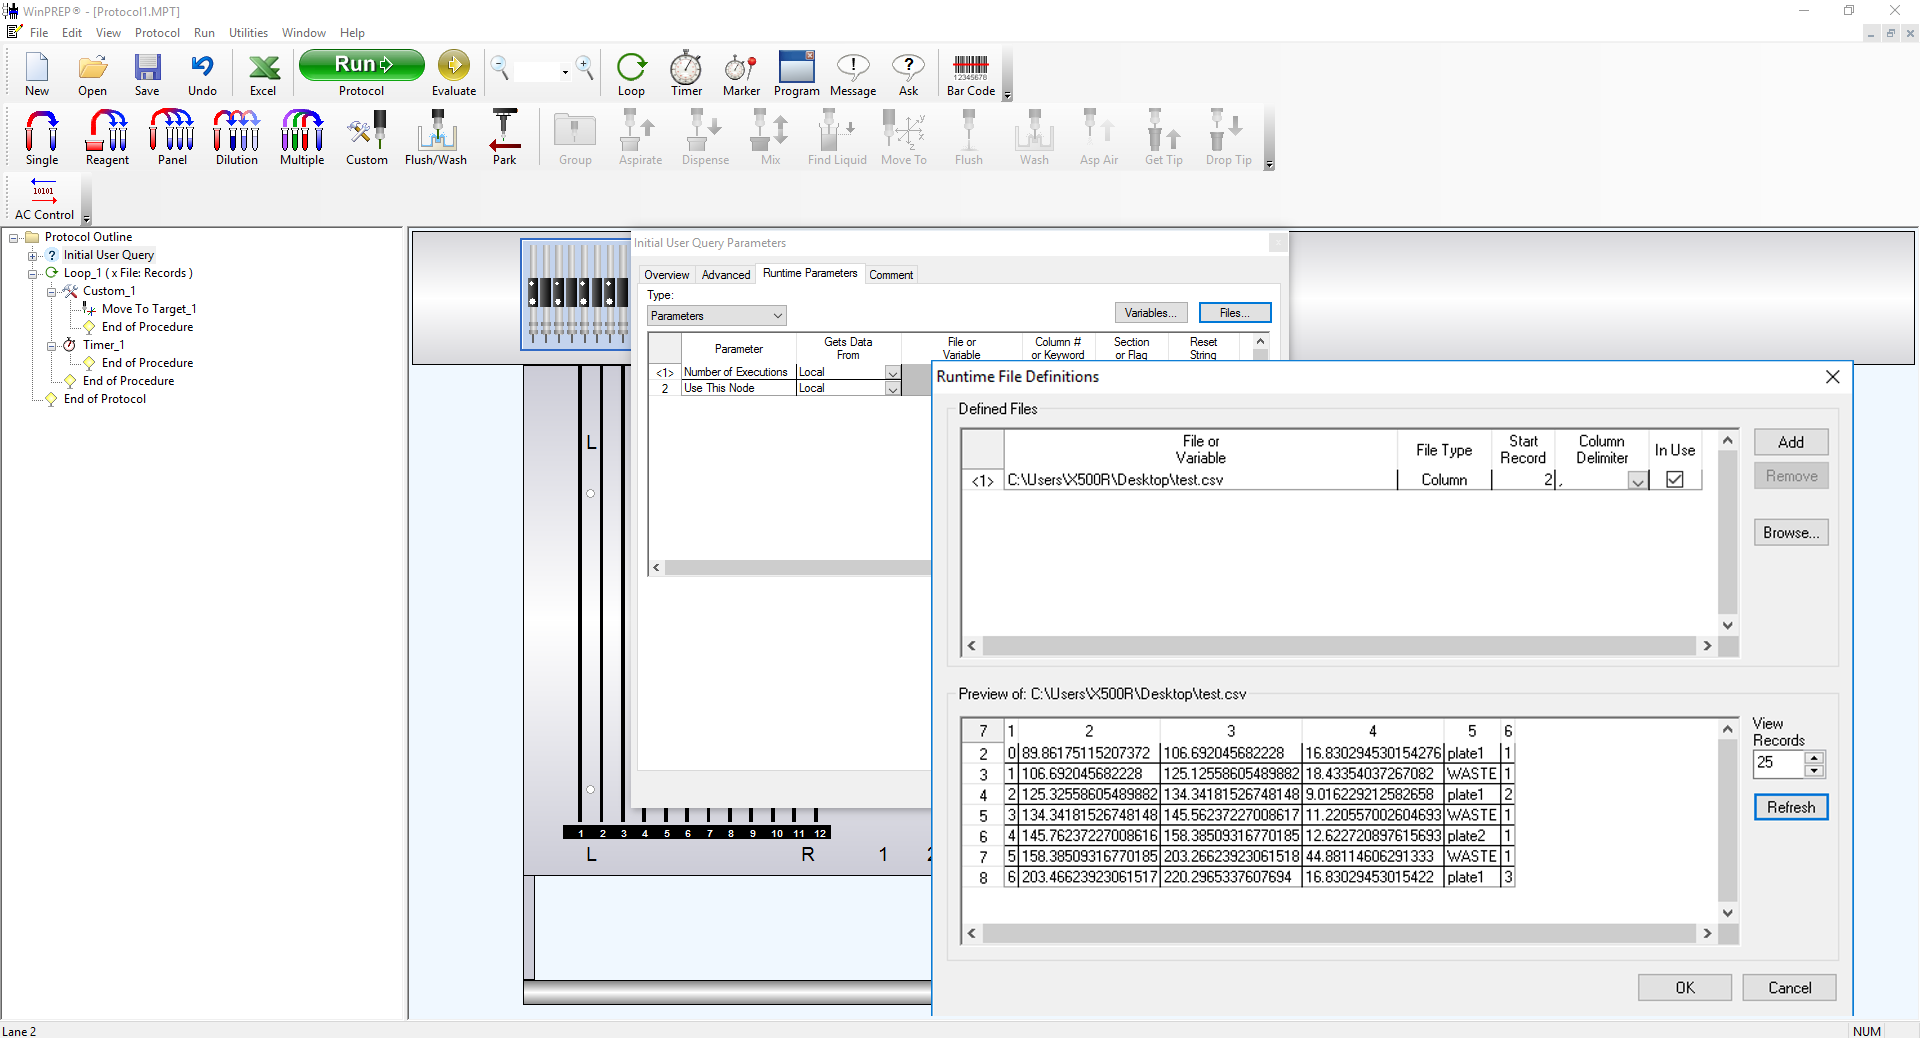
\includegraphics[width=\textwidth]{assets/1.png}
        \caption{Primer generirane CSV datoteke z destinacijam, uporabljene v WinPREP}
        \label{fig:csv_output}
\end{figure}

\subsection{Prikaz in dostop podatkov}
Na prvi pogled se prikaz zajetih podatkov kot slike zdi nenavadno, vendar so za to implementacijo tehtni razlogi. Za prikaz grafikonov so potrebni "surovi" podatki, toda programski platformi SciexOS in Analyst hranita podatke v "zaprtokodnih" datotekah formata .wiff/2. Trenutno priznane alternative  za procesiranje teh datotek ni. Program ProteoWizard\cite{proteo} sicer ponuja CLI orodje, ki s sklici na funkcije v uradnih programskih knjižnicah (dll) pretvori v .mzML format. Ta pristop se sprva zdi obetaven, toda hitro sem se srečal z vrsto problemov.

Prvič, ProteoWizard podpira takšno pretvorbo le na Windows platformi, katero podpira proizvajalec, Sciex. Drugi problem je v nastalih .mzML datotekah – po dolgem procesiranju pridobimo datoteke, ki so nekaj magnitud večje kot originalne, zgščene vendorske datoteke (15MB $\rightarrow$ 1.5GB). Seveda nisem prvi, ki je naletel na ta problem; na trgu se je že pojavilo več odprtokodnih formatov\cite{toffee} za učinkovito hrambo ToF/Swath-ms podatkov (Toffee in drugi). Navkljub prvotnemu upanju se žal tudi uporaba te knjižnice ni izkazala za rešitev. Da bi pridobili naše podatke, bi jih morali spraviti skozi več stopenj procesiranja (še vedno bi se najprej ustvarila mzML datoteka, šele nato Toffee), kar bi dodalo nesprejemljiv zagonski (load) čas, še posebej opazen na počasnem računalniku, uporabljenem za nadzor laboratorijskih naprav. Uporaba slike je zato trenutno najbolj ekonomična rešitev.

Zaradi istega razloga nisem implementiral t.i. avtomatične zaznave lokalnih maksimumov. Eksperimentiral sem z različnimi funkcijami za zaznavo in se spoznal tudi z različnimi orodji ter knjižnicami\cite{pymassspec}, ki podpirajo naprednejše algoritme, kot je adaptivni algoritem za iskanje maksimov (AMPD - Automatic Multiscale-based Peak Detection), ki je posebej zasnovan za zaznavo vrhov v časovnih serijah z različnimi frekvenčnimi komponentami. V primeru, da bi bili na voljo surovi podatki, bi bila dodaja avtomatske zaznave trivialna. Saj bi lahko v tem primeru uporabil detekcijo signala kot je prikazano spodaj.
\begin{lstlisting}[caption={Uporaba Savitzky-Golay filtra za glajenje šuma, pri detekciji peak-ov}, label={lst:filters}]
from scipy.signal import savgol_filter

def d_peak_detection(x, y, window_size=15, polyorder=3, prominence=0.1):
    y_smooth = savgol_filter(y, window_size, polyorder)
    dy = np.gradient(y_smooth)
    
    zero_crossings = np.where(np.diff(np.signbit(dy)))[0]
        peaks = []
    for idx in zero_crossings:
        if y_smooth[idx] > prominence * np.max(y_smooth):
            peaks.append((x[idx], y_smooth[idx]))
    return peaks
\end{lstlisting}
\section{Zaključek}

Program, ki sem ga razvil, uspešno rešuje zastavljeni problem označevanja interesnih vrhov na spektrogramu in generiranja kontrolnih datotek za robotsko pipetiranje. Programska koda je modularna in prilagodljiva, kar omogoča enostavno nadgradnjo z novimi funkcionalnostmi.

Glavne prednosti programa so enostavna uporaba, prilagodljivo časovno skaliranje in uporabniku prijazno označevanje interesnih regij. Poleg tega program avtomatsko ustvarja vmesne "WASTE" pozicije med označenimi regijami in kompenzira za časovne zamike pri robotskih premikih.

Če se bo pokazala potreba, bom program izboljšal z natančnejšim sistemom za kompenzacijo časovnih zamikov, neposredno integracijo z WinPREP API-jem in implementacijo avtomatske zaznave vrhov, ko bodo na voljo surovi podatki v dostopnem formatu.

Ta projekt prikazuje, kako lahko z uporabo odprtokodnih orodij in programskih jezikov razvijemo specifične rešitve za laboratorijske potrebe, ki bi bile sicer drage ali nedostopne preko komercialnih ponudnikov.

\begin{figure}[H]
    \centering
    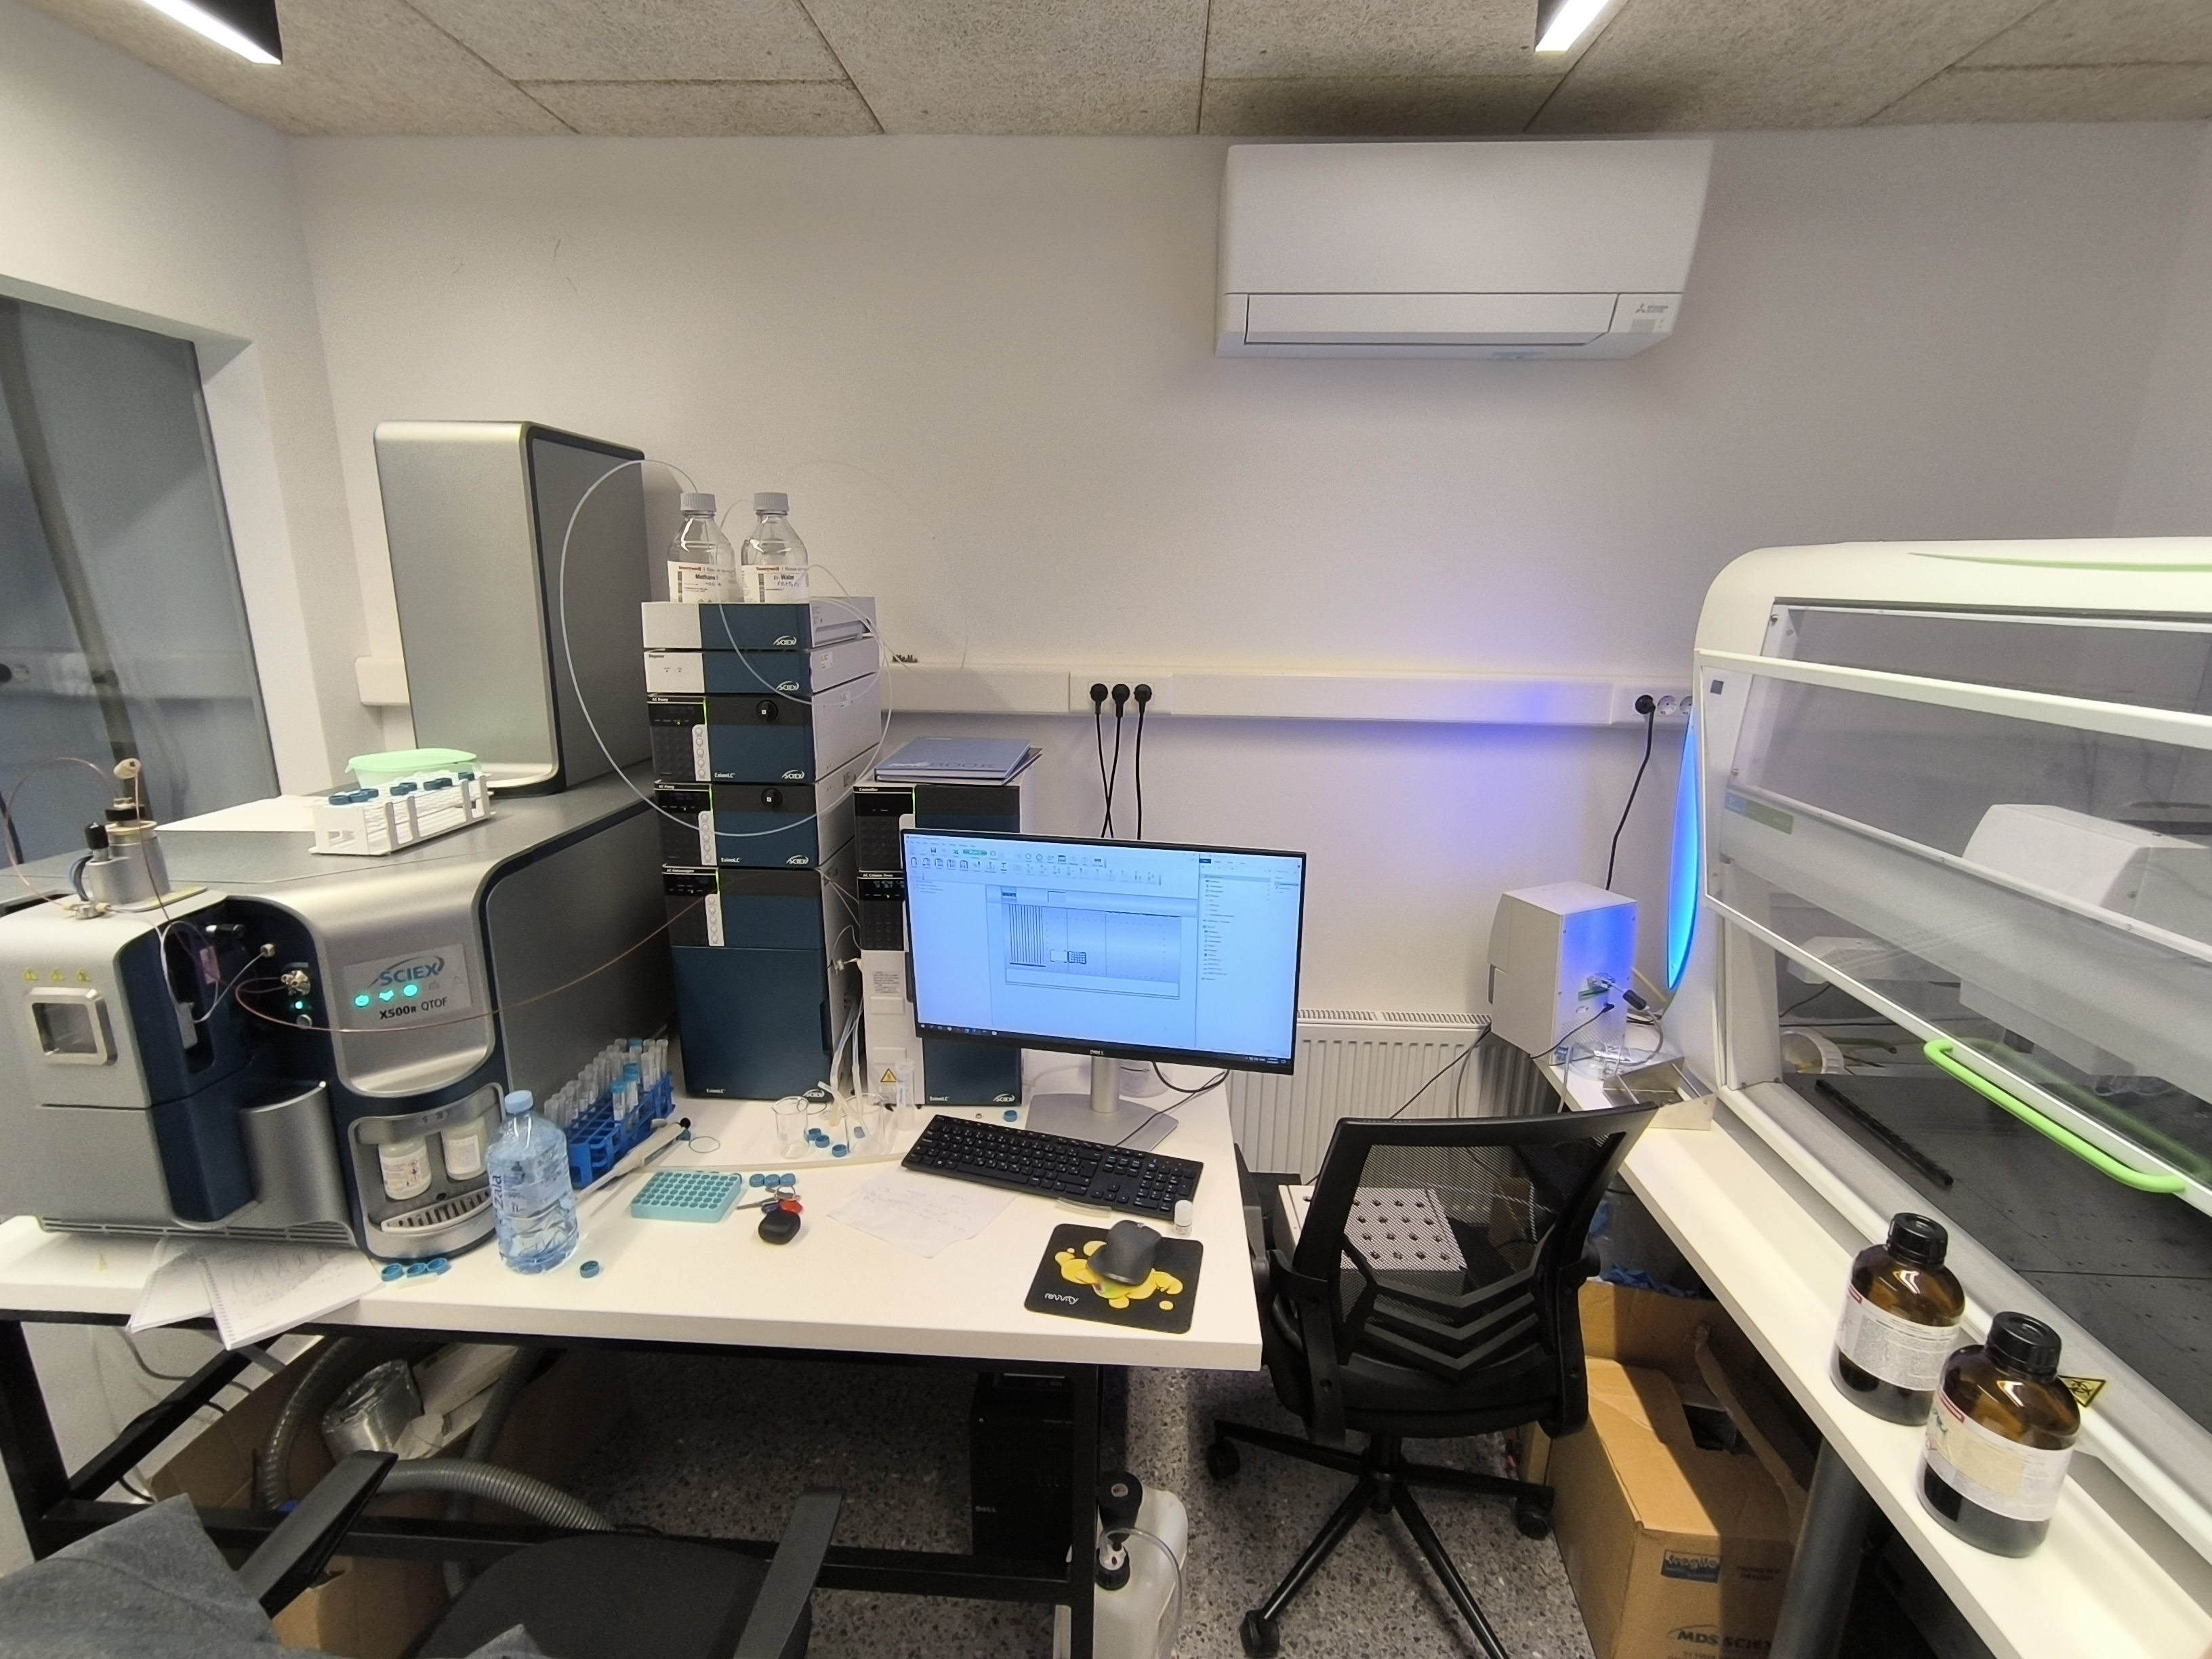
\includegraphics[width=0.9\textwidth]{assets/ermmm.jpg}
    \caption{Prikaz delovanja programa s pravim masnim spektrometrom in JanusG3 robotom v laboratorijskem okolju.}
    \label{fig:real_lab_application}
\end{figure}
\newpage
\appendix
\section{Izvorna koda programa}
Izvorna koda je dostopna na git repozitoriju \url{https://github.com/marwuint/gawr}. 
%\lstinputlisting[caption={Celotna izvorna koda programa}]{source_code.py}
\section{Viri}
\begin{thebibliography}{9}
\bibitem{matplotlib}Ustvarjalci Matplotlib. (2025). \textit{Matplotlib: Python plotting}. \url{https://matplotlib.org/}

\bibitem{tkinter} Python Software Foundation. \textit{tkinter — Python interface to Tcl/Tk}. Python Documentation. \url{https://docs.python.org/3/library/tkinter.html}

\bibitem{pandas}Ustvarjalci pandas. (2025). \textit{pandas: powerful Python data analysis toolkit}. \url{https://pandas.pydata.org/}

\bibitem{nspanselector} PyNexafs. (2025). \textit{NSpanSelector implementation}. GitHub Repository. \url{https://github.com/xraysoftmat/pyNexafs/blob/910bd5e3aef113696ebdcce207e45de8d0a945e9/pyNexafs/gui/widgets/graphing/matplotlib/widgets.py}

\bibitem{pymassspec} PyMassSpec Team. \textit{Peak Detection and Representation}. \url{https://pymassspec.readthedocs.io/en/master/40_peak_detection_and_representation.html}

\bibitem{toffee} Tully B. (2020). \textit{Toffee - a highly efficient, lossless file format for DIA-MS}.  Scientific reports, 10(1), 8939. \url{https://pmc.ncbi.nlm.nih.gov/articles/PMC7265431/}

\bibitem{proteo}Ustvarjalci ProteoWizard. \textit{msconvert a command line tool for converting between various file formats.}. \url{https://proteowizard.sourceforge.io/}\
\end{thebibliography}
\newpage
\section*{Izjava o avtorstvu}
\begin{minipage}{0.8\textwidth}
Izjavljam, da je ta seminarska naloga v celoti moje avtorsko delo, pripravljeno s pomočjo navedene literature in pod vodstvom mentorja.
\vspace{1.2cm}

\noindent\rule{7cm}{0.4pt}\\
Martin Hanzlowsky
\thispagestyle{empty}
\end{minipage}
\end{document}